\section{System Design}
\label{sec:system-design}

\subsection{System Overview}
\label{subsec:system-overview}

\subsubsection*{Engine Design}

The project's core engine design, as stated before, will use an ECS framework that registers and
determines components and system dependencies at compile-time.
The declaration of a single ECS instance that registers all components and systems would result in
wasteful usage of memory and projected performance decreases due to the large variety of components involved.
As such, we have opted to use multiple smaller ECS instances that each take control of a smaller part of the game.
We refer to these smaller ECS instances, alongside the data necessary to register related components and systems,
as well as compute and store initial data into those instances, as scenes.
Communications between scenes, such as the data transfer when creating a new scene, are facilitated through
a manager, which will also execute the registered systems during the main game loop.
DirectX 11 is used for the rendering of the game with the use of a custom rendering pipeline implementation.
User input is collected through the Windows API\@.

For the actual implementation of these compile-time optimizations, we take advantage of C++'s concept of templates.
By using component and system data types as template parameters, we can use template specialization to let
the compiler generate code specific to our use case.
Since each system is a function, this also means we get usage of functions without relying on indirect calls,
which is a common pain point in engine design.
\\\\
The benefits of template specialization can be seen with a key part of the ECS instance, the resource manager.
The resource manager manages entities along with any components attached to those entities, together referred to as resources.
The resource manager takes a size integer and any number of structures as template parameters and treats those
structures as registered components in this instance.
It will create a resource pool of each registered component with the specified size when constructed, each of
which will reserve their own memory depending on the component's size and the pool size.
By accessing these components through template specialization, code is generated such that the abstraction layers
are removed from the code when compiled.
\\\\
While systems are being run, entities with select component archetypes are iterated upon.
If components are added or removed during iteration, this may invalidate references or otherwise cause unpredictable behavior.
To avoid such hazards, a structure must be created with the purpose to defer all attempts to add or remove components
and to apply such changes after all systems complete execution.
Borrowing the term from operating systems, we refer to this structure with elevated permissions to modify resources
as the syscall.
The syscall must know the components registered to its coupled resource manager so that it can add the appropriate
components.
When systems want to add or remove components from an entity, they make the request to the ECS instance, which
will schedule the changes in its internal syscall.
\\\\
Systems operate upon entities based on whether they fulfill certain component requirements.
For complex systems, the requirements can be rather complex, and entities may be retrieved multiple times
under different requirements.
Some implementations have the ECS instance be provided as a function argument to each system so that entities
can be retrieved directly from internal resources via templated retrieval functions.
We decided, instead, that systems define query data structures as function arguments, which describes the components
that entity references stored within are guaranteed to possess.
When the system is run, the ECS instance will internally fulfill each query requirement by fetching and filtering
from the resource manager before passing them to the system.
This way, the system's implementation does not concern itself with fetching data from the ECS instance.

\subsubsection*{Game Design}

The project’s core game design will involve combining rhythm games and bullet hell games into a hybrid game
structured around distinct but smoothly transitioning phases,
thus requiring a seamless transition between the two, creating a revolutionary take on hybrid games.
Having that both of the games hugely relied on great optimization, as with a little disruption,
it can cause a fatal unintended mistake for the player inciting frustration;
therefore, the design of the game must be made cautiously.
\\\\
The bullet hell section is mostly composed of large amounts of bullets and particles
while great performance is still required to attain the player’s fluidity of movement.
To achieve this, an ECS architecture is highly favoured as opposed to object-oriented
since the high amount of entities can be handled more efficiently with it.
Entities of the system are composed of player, bullets, boss, enemies, background and effects
utilizing shared components such as position, velocity, sprite, shader, etc.
Each system will be executed every frame thus handling the entity movement,
collision check and input allowing it to handle all the bullets in a frame efficiently.
Such systems consist of a player system, movement system, collision system, particle system and much more.
The core mechanics is for each frame, the input was processed to control the player system
while the collision system will check each ongoing colliding entity by calling each entity with a collider component
and computing if they are colliding with which entity.
Then, the corresponding function will be triggered to apply change to the state such as the player taking damage and making change to the player’s health UI\@.
Moreover, the movement system computes the next frame position to render, and lastly, the animation system will render the right frame of the animation at the correct time.
\\\\
Rhythm games require precise timing and precision to catch the note at the right time,
very little or next to none of the optimization issues can be tolerated as a result.
However, ECS architecture is powerful enough to handle all the requirements
such as notes quantities and an accurate time tracking device centralized by a single system.
With entities as simple as notes, lanes and judgement, components are widely adjustable with speed, timing and judgement.
In addition, the system design is fairly simple as the input system and judgement system is centralized and the note system moves all notes called.
Along with the bullet hell section, they contain backgrounds that are adjustable by shader and particle effects.
The core mechanic revolves around spawning the notes at the right time as set up.
Then, each note will be called by the movement system to calculate the position of the sprite.
However, the real logic of the note is being computed by another system that reduces its timing to be compared in the judgement system.
Lastly, the judgement system calls the corresponding system to handle whether if the note has been well-time pressed and sending responses to the player.
\\\\
Transitioning between both gameplay proves to be a great challenge design-wise
because it has to be smooth and seamless enough to not disrupt the precision-hungry gameplay of both games.
Firstly, in the whole game process, only one game scene may be rendered to minimize time to transition
as the whole scene will be loaded and initiated only once from the start.
If the transition is happening, the gameplay should be frozen and any progress should not be counted during the process,
allowing the player to get ready to adjust their gameplay smoothly.
The transition's animation has to telegraph the player clearly to make them aware that the gameplay is going to be changed
as the timer UI counts down to inform the duration and delay of the transition precisely.
Lastly, the screen changing the gameplay rendered has to be transition creative by splitting the screen in two and slowly expanding the next gameplay.
To achieve this, a line animation system is used to express animation of the transition
and the Game Transition System will be triggered if the state has been changed rendering the new gameplay for a section of the screen expanding until full.
\\\\
A biggest concern of the system is the control of the rhythm game’s charts and bullet hell’s patterns
needing to be not too exhaustingly difficult to control as both games require vast amounts of complicated pattern and timing design.
A solution proposed would be to create our own scripting language and a corresponding compiler such as a chart file.
Practicing these techniques makes designing and implementing charts and patterns much easier
allowing more complex and challenging design and features.
\\\\
To complete a game, a narrative device should be implemented to make the game more immersive and enjoyable;
the proposed gameplay would be a 2D side-scrolling style that allows players to choose a level and progress the story of the gameplay.
Additionally, explorations are added to the game such as interacting with an interactable such as NPC, or objects, obtaining new in-game items and accessing new areas.
Such requirements must be implemented with an entirely new system.
Interactable and solid collision components are needed to be implemented along with the new system, for example, new movement system, interact system and area load system.
\\\\
Lastly, using ECS, UI entities are being rendered concurrently in a higher priority by default.
The entities will have a position, text, sprite and animation components and are created organizedly using functions for each set of UIs.
For sound and music in the game, just like UIs as each is assigned to its own entity holding a tag or trigger to be played on an instance sound system at the right time.
Finally, the cutscene could be added as a video format to be rendered in an instance video player system.



\subsection{Components}
\label{subsec:components}

The system is a self-contained application, but interfacing with a keyboard and mouse is required for its operation.



\subsection{Constraints Considered}
\label{subsec:constraints-considered}

Due to the usage of the Windows API and DirectX 11, the system is to be operated and published only on
the Windows operating system.

\subsection{Diagrams}
\label{subsec:diagrams}

\vspace{0.5cm}

\begin{figure}[h]
    \centering
    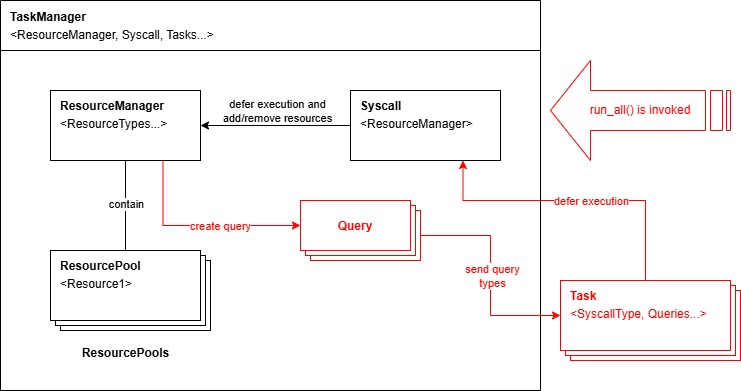
\includegraphics[width=\columnwidth, keepaspectratio]{images/taskmanager}
    \caption{A diagram showing how task manager works}
    \label{fig:taskmanager}
\end{figure}

\vspace{0.5cm}

\noindent Figure~\ref{fig:taskmanager} shows the composition of the task manager, a unit of ECS instance.
Using template instantiation, the task manager knows the type of its resources(components) and tasks(systems),
and creates the required storage and functionality when constructed.
When the task manager receives a signal to advance its state, depending on the type of task, it will
formulate the appropriate queried resource data structure and apply it as a parameter to its registered tasks.
The tasks state the query requirements in advance so that this process can be inferred at compile-time.

\vspace{0.5cm}

\begin{figure}[h]
    \centering
    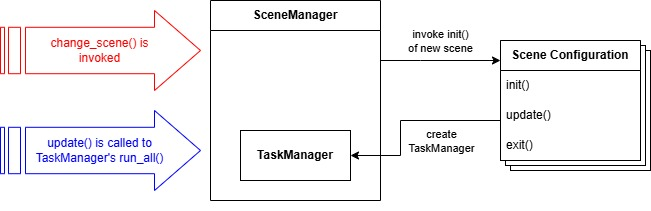
\includegraphics[width=\columnwidth, keepaspectratio]{images/scenemanager}
    \caption{A diagram showing how scene manager works}
    \label{fig:scenemanager}
\end{figure}

\vspace{0.5cm}

\noindent Figure~\ref{fig:scenemanager} shows the composition of the scene manager, which manages ECS instances.
The scene manager registers a collection of scenes in advance, where each scene is a data structure with the
functions to create a task manager instance.
When the scene manager chooses a scene to change to, the scene's functions are invoked, returning the created
task manager instance to the scene manager to update during the game loop.

\vspace{0.5cm}

\begin{figure}[h]
    \centering
    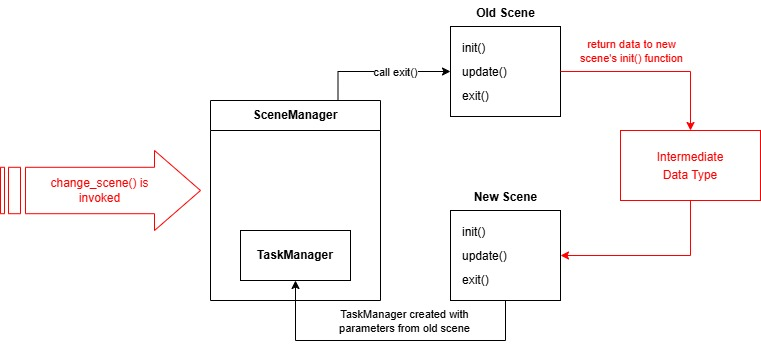
\includegraphics[width=\columnwidth, keepaspectratio]{images/scenemanager2}
    \caption{A diagram showing how scene manager transfers data from old scene to new scene}
    \label{fig:scenemanager2}
\end{figure}

\vspace{0.5cm}

\noindent When the game logic leaves one scene and enters another, persistent data between scenes may be required.
The operation of this data transfer is shown in Figure~\ref{fig:scenemanager2}.
As shown, when a scene is exited, it returns an intermediate data structure containing the data of resources
it wishes to transfer to the next scene.
This data structure is then applied as arguments for initialization of the scene to enter.
\\\\
Through the functionality of the task manager and scene manager, the assembly and disassembly of memory-efficient
ECS instances with complete knowledge of required data types can be achieved without losing any functionality of
single-instance ECS implementations.

\vspace{0.5cm}

\begin{figure}[h]
    \centering
    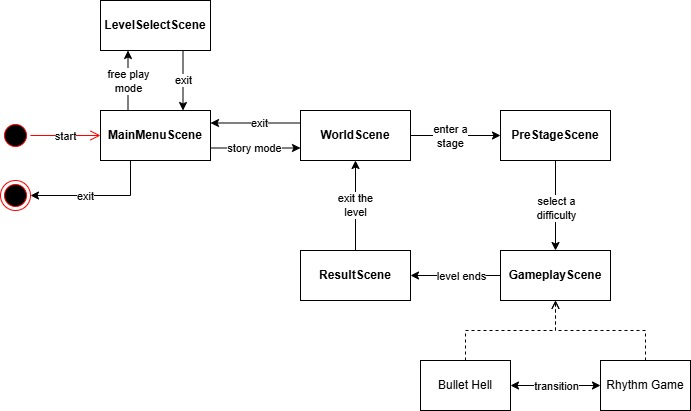
\includegraphics[width=\columnwidth, keepaspectratio]{images/gameflow}
    \caption{A diagram showing scene flow of the game prototype}
    \label{fig:gameflow}
\end{figure}

\vspace{0.5cm}

\noindent Figure~\ref{fig:gameflow} shows how the scenes in our game should flow.
The game starts from the main menu scene where the player can choose to enter the game or exit.
After the player chooses to enter the game, the game's world scene will be loaded.
There will be objects across the world which act as stages that the player can interact with to 
enter the level.
When the player interacts with a stage object, the game will transition to pre-stage scene, where 
they can select which instrument to use in the level.
Each instrument represents a different difficulty level.
The player can choose to start the level with the selected instrument or return to the world.
\\\\
Once the player starts the level, the game will transition to the main gameplay scene.
The gameplay scene consists of both bullet hell and rhythm game phases.
In this scene, as the level begins, the player will start with bullet hell phase.
The player must avoid incoming obstacles from the enemy and survive throughout the phase.
If the player's health reaches zero at any point, the gameplay will end, failing the level.
After surviving the for a certain amount of time, the game will transition to rhythm game phase.
In this phase, the player must hit the notes in time with the music to attack the enemy.
Each successful note hit will slightly fill the enemy's gauge and heal the player, while missed notes will 
only deplete the gauge.
The player must fill the gauge above a certain threshold to defeat the enemy and complete the level.
Then, the game will transition back to bullet hell phase again.
This cycle continues until the song ends or the player is defeated first.
If the player successfully fills the gauge above the threshold by the end of the song, the player wins.
Otherwise, it is considered a draw.
\\\\
After the gameplay ends, regardless if the player wins, loses or draws, the game will transition to results 
scene, displaying the player's performance statistics.
Then, the player will return to the world scene to continue exploring or choose another level.